% =====================================================================
%  9. Résultats semi-supervisés : COREG
% =====================================================================
\clearpage
\section{Résultats semi-supervisés : COREG}
\label{sec:ssl}

COREG (\cref{subsec:coreg_algo}) a été entraîné dans le notebook
\notebook{07\_coreg.ipynb} pour les trois cibles de traction, avec la
configuration 16/médiane, sous les deux protocoles de validation imbriquée et selon
le protocole inductif de la \cref{subsec:inductif}. Tous les vrais labels du train
sont utilisés ; aucun label n'est masqué artificiellement. Charpy n'est pas
concerné, son pool naturel étant vide. Au total : 180 évaluations externes et
576 ajustements COREG (choix internes, réapprentissages complets et sensibilité
aux graines compris).

\subsection{Méthodes comparées}

Pour attribuer correctement un éventuel gain aux pseudo-labels, COREG est comparé
à plusieurs contrôles évalués sur exactement les mêmes observations :
\begin{itemize}
  \item \textbf{moyenne $k$NN L1/L2 au même $k$, sans pseudo-labels} : le contrôle \emph{apparié}, qui ne diffère de COREG que par l'ajout de pseudo-labels ;
  \item \textbf{moyenne $k$NN L1/L2 réglée} : même architecture, $k$ choisi indépendamment ;
  \item \textbf{$k$NN L1 seul} et \textbf{$k$NN L2 seul} ;
  \item \textbf{sélection supervisée} : la procédure de référence de la \cref{subsec:res16}, qui ne sert jamais à initialiser COREG.
\end{itemize}

\subsection{Déroulement de la boucle}

Le \cref{tab:coreg_boucle} résume ce qui se passe dans les cinq ajustements
externes de chaque cible et protocole.

\begin{table}[htbp]
\centering
\small
\caption{Déroulement de COREG dans les cinq plis externes (min--max sur les plis).
\og Pool distinct \fg{} : après déduplication et retrait des représentations déjà
présentes parmi les vrais labels.}
\label{tab:coreg_boucle}
\footnotesize
\setlength{\tabcolsep}{4pt}
\begin{tabular}{@{}l l rrrr l@{}}
\toprule
Protocole & Cible & Pool brut & Pool distinct & Pseudo-labels & Tours & Arrêts \\
\midrule
Aléatoire & \YS     & 679--680 & 224--234 & 118--170 & 61--91 & 5 sans gain positif \\
          & \UTS    & 702--703 & 249--258 & 70--158  & 38--82 & 5 sans gain positif \\
          & Allong. & 739--740 & 275--290 & 52--197  & 29--100 & 4 sans gain, 1 au maximum \\
\midrule
Groupé    & \YS     & 651--696 & 143--240 & 80--200  & 42--100 & 2 sans gain, 2 max., 1 pool épuisé \\
          & \UTS    & 682--742 & 149--270 & 122--200 & 66--100 & 3 sans gain, 2 au maximum \\
          & Allong. & 725--763 & 189--293 & 80--200  & 42--100 & 2 sans gain, 3 au maximum \\
\bottomrule
\end{tabular}
\end{table}

La déduplication réduit fortement le pool : sur environ 700 lignes sans label par
pli, seules 140 à 290 représentations sont réellement nouvelles. Beaucoup de
lignes non étiquetées décrivent des conditions déjà présentes parmi les labels.
La \cref{fig:coreg_iter} montre que chaque tour ajoute presque toujours deux
pseudo-labels (un par régresseur) jusqu'à l'arrêt.

\begin{figure}[htbp]
\centering
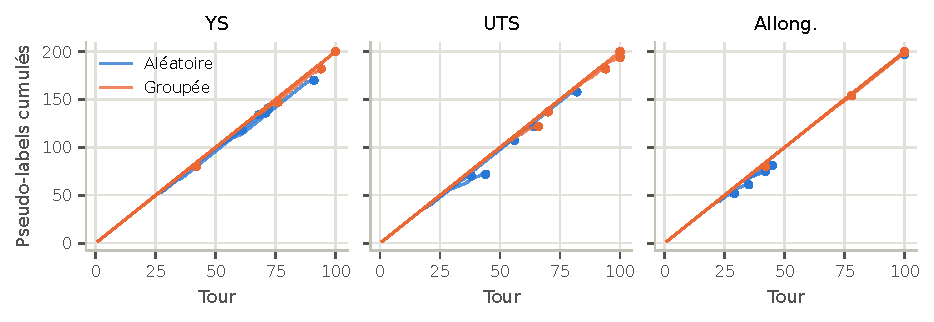
\includegraphics[width=\textwidth]{coreg_iterations}
\caption{Nombre cumulé de pseudo-labels acceptés au fil des tours, pour chacun des
cinq plis externes (un trait par pli ; point : arrêt). La croissance est
quasi linéaire (deux ajouts par tour) jusqu'à l'absence de gain positif ou au
plafond de 100 tours.}
\label{fig:coreg_iter}
\end{figure}

\subsection{Performances}

\begin{figure}[htbp]
\centering
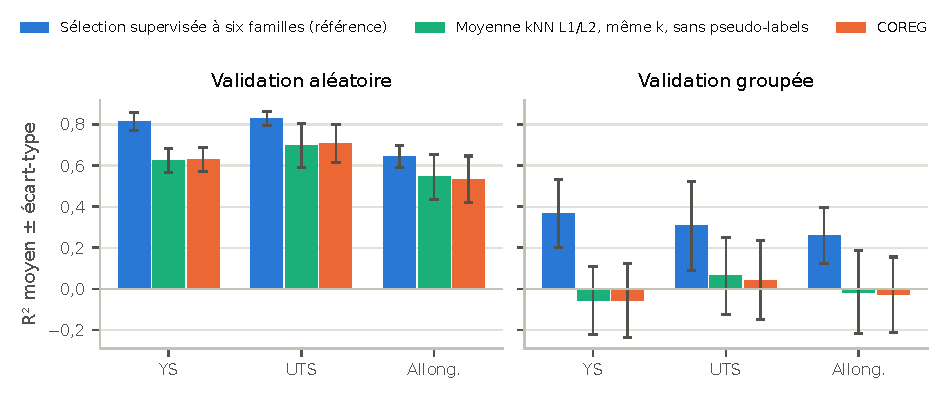
\includegraphics[width=\textwidth]{coreg_comparaison}
\caption{$R^2$ moyen ($\pm$ écart-type) de COREG, de son contrôle apparié sans
pseudo-labels et de la sélection supervisée de référence.}
\label{fig:coreg_comp}
\end{figure}

\begin{table}[htbp]
\centering
\small
\caption{COREG et contrôles : MAE moyenne et $R^2$ moyen sur les cinq plis externes.}
\label{tab:coreg_res}
\setlength{\tabcolsep}{4pt}
\begin{tabular}{@{}l l rr rr rr rr@{}}
\toprule
 & & \multicolumn{2}{c}{COREG} & \multicolumn{2}{c}{$k$NN même $k$} & \multicolumn{2}{c}{$k$NN réglés} & \multicolumn{2}{c}{Supervisé (réf.)} \\
\cmidrule(lr){3-4}\cmidrule(lr){5-6}\cmidrule(lr){7-8}\cmidrule(lr){9-10}
Protocole & Cible & MAE & $R^2$ & MAE & $R^2$ & MAE & $R^2$ & MAE & $R^2$ \\
\midrule
Aléatoire & \YS{} (MPa)   & 37,919 & 0,629 & 38,241 & 0,625 & 38,241 & 0,625 & \meilleur{31,630} & \meilleur{0,755} \\
          & \UTS{} (MPa)  & 33,037 & 0,709 & 33,319 & 0,698 & 33,319 & 0,698 & \meilleur{23,861} & \meilleur{0,836} \\
          & Allong. (pts) & 2,402  & 0,535 & 2,392  & 0,546 & 2,392  & 0,546 & \meilleur{2,054}  & \meilleur{0,660} \\
\midrule
Groupé    & \YS{} (MPa)   & 71,074 & $-0{,}056$ & 70,817 & $-0{,}055$ & 71,717 & $-0{,}080$ & \meilleur{56,757} & \meilleur{0,337} \\
          & \UTS{} (MPa)  & 63,060 & 0,043 & 62,081 & 0,064 & 62,081 & 0,064 & \meilleur{54,344} & \meilleur{0,334} \\
          & Allong. (pts) & 3,904  & $-0{,}028$ & 3,879 & $-0{,}015$ & 3,879 & $-0{,}015$ & \meilleur{3,517} & \meilleur{0,157} \\
\bottomrule
\end{tabular}
\end{table}

\subsection{Gain apparié et robustesse}

Le gain apparié compare COREG et le contrôle au même $k$ sur les mêmes
prédictions hors pli (gain positif = COREG réduit la MAE). L'intervalle est un
bootstrap descriptif par séries (2\,000 tirages).

\begin{table}[htbp]
\centering
\small
\caption{Gain de MAE OOF de COREG par rapport au contrôle apparié (même $k$, sans
pseudo-labels) et par rapport à la sélection supervisée.}
\label{tab:coreg_gain}
\begin{tabular}{@{}l l r l r l@{}}
\toprule
 & & \multicolumn{2}{c}{vs $k$NN même $k$} & \multicolumn{2}{c}{vs supervisé} \\
\cmidrule(lr){3-4}\cmidrule(lr){5-6}
Protocole & Cible & Gain & Intervalle 95\,\% & Gain & Intervalle 95\,\% \\
\midrule
Aléatoire & \YS     & 0,322    & [$-0{,}060$ ; 0,782]   & $-6{,}287$  & [$-11{,}367$ ; $-2{,}070$] \\
          & \UTS    & 0,283    & [$-0{,}154$ ; 0,886]   & $-9{,}175$  & [$-15{,}279$ ; $-3{,}679$] \\
          & Allong. & $-0{,}011$ & [$-0{,}035$ ; 0,013] & $-0{,}349$  & [$-0{,}637$ ; $-0{,}011$] \\
\midrule
Groupé    & \YS     & $-0{,}272$ & [$-1{,}144$ ; 0,523] & $-14{,}245$ & [$-21{,}023$ ; $-6{,}827$] \\
          & \UTS    & $-0{,}920$ & [$-1{,}939$ ; $-0{,}275$] & $-7{,}721$ & [$-18{,}425$ ; 3,331] \\
          & Allong. & $-0{,}024$ & [$-0{,}106$ ; 0,029] & $-0{,}382$  & [$-0{,}780$ ; $-0{,}023$] \\
\bottomrule
\end{tabular}
\end{table}

\paragraph{Lecture des résultats.}
\begin{itemize}
  \item \textbf{Effet propre des pseudo-labels.} En aléatoire, COREG améliore très légèrement la MAE pour \YS{} (0,32\,MPa) et \UTS{} (0,28\,MPa), mais les intervalles couvrent zéro. En groupé, les trois gains sont négatifs, et celui d'\UTS{} est entièrement négatif ([$-1{,}94$ ; $-0{,}28$]\,MPa).
  \item \textbf{Comparaison à la référence.} COREG est moins bon que la sélection supervisée dans \textbf{les six cas}, de 6 à 14\,MPa sur la résistance.
  \item \textbf{Graines.} Avec les graines de base 43 et 44 et le même $k$, les MAE varient de moins de 0,5\,MPa (par exemple \UTS{} aléatoire : 33,04 ; 32,98 ; 33,31) : la conclusion ne dépend pas du tirage des candidats.
\end{itemize}

\subsection{Pourquoi COREG n'apporte-t-il pas de gain ici ?}

Plusieurs explications sont cohérentes avec les mesures, sans qu'aucune ne soit
isolée comme cause unique :
\begin{enumerate}
  \item \textbf{Le régresseur de base est faible hors série.} Les $k$NN sans pseudo-labels ont déjà un $R^2$ proche de zéro en groupé. COREG ne peut que \emph{propager} leurs estimations ; il ne crée pas l'information physique manquante qui permettrait de corriger un décalage entre séries.
  \item \textbf{Le pool apporte peu de diversité.} Après déduplication, seule une fraction du pool est nouvelle, et ces lignes proviennent des mêmes séries que les labels.
  \item \textbf{La confiance est locale.} Le gain $\Delta_u$ mesure la cohérence d'une estimation avec ses voisins étiquetés, pas son exactitude ; les deux $k$NN partagent les mêmes entrées et peuvent renforcer une erreur commune.
  \item \textbf{Le budget de labels est complet.} Le semi-supervisé est surtout utile lorsque les labels sont rares ; ici tous les labels disponibles sont utilisés. Un scénario à 25 ou 50\,\% de labels serait une expérience distincte.
\end{enumerate}

\subsection{Modèles exportés}

Une nouvelle CV5 sur tous les labels (aléatoire graine 1042, ou par groupes) a
choisi $k$ pour les réapprentissages complets : $k = 3$ pour les trois cibles en
aléatoire (82, 44 et 41 pseudo-labels ajoutés), $k = 15$, 5 et 3 en groupé pour
\YS, \UTS{} et l'allongement (200, 186 et 14 pseudo-labels). Au total
\textbf{108 pipelines} sont exportées (90 de plis externes et 18 complètes,
contrôles inclus). Un audit indépendant a recalculé les 180 scores, vérifié
l'isolement des données pour les 576 ajustements et leurs 81\,931 pseudo-labels,
et recalculé explicitement 1\,410 gains.

\begin{aretenir}
COREG a été mis en œuvre selon un protocole inductif rigoureux et comparé à son
exact pendant supervisé. Il \textbf{n'apporte pas de gain significatif} : gains
de l'ordre de 0,3\,MPa non significatifs en aléatoire, gains négatifs en groupé,
et il reste nettement en dessous de la sélection supervisée dans tous les cas.
Les modèles supervisés restent la référence pour cette base.
\end{aretenir}
